\documentclass[convert, tikz]{standalone}
\usepackage{tikz}
\usetikzlibrary{arrows, backgrounds, calc, decorations.pathreplacing, fit, positioning, shapes.geometric}
\pagecolor[RGB]{255,255,255}
\begin{document}
 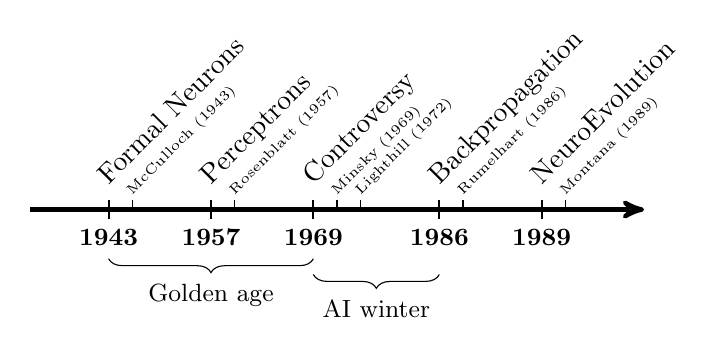
\begin{tikzpicture}[>=stealth']
  \def\x{0}
  \tikzset{
   label/.style={rotate=45, text depth=0pt, text height=0pt},
   minor/.style={label, font=\tiny, inner sep=.1em},
   major/.style={label},
  }
  \foreach \title/\year/\flag [count=\i from 0] in {
   Formal Neurons/1943/1,
    McCulloch/1943/0,
   Perceptrons/1957/1,
    Rosenblatt/1957/0,
   Controversy/1969/1,
    Minsky/1969/0,
    Lighthill/1972/0,
   Backpropagation/1986/1,
    Rumelhart/1986/0,
   NeuroEvolution/1989/1,
    Montana/1989/0
  } {
   \ifnum\flag=0
    \def\t{}
    \def\style{minor}
    \def\dx{.3}
    \def\text{\title\ (\year)}
    \def\p{(\x, 0) -- ++(0, .125)}
   \else
    \def\t{thick}
    \def\style{major}
    \def\dx{1}
    \def\text{\title}
    \def\p{(\x, -.125) -- ++(0, .25)}
   \fi
   \pgfmathsetmacro{\x}{\x+\dx}
   \draw [\t] \p node [anchor=south west, \style] {\text};
   \ifnum\flag>0
    \node at (\x, -.125) [anchor=north] {\small\textbf{\year}};
    \coordinate (\i) at (\x, -.125);
   \fi
   \xdef\x{\x}
  }

  \foreach \s/\e/\l [count=\i] in {
   0/4/Golden age,
   4/7/AI winter
  } {
   \pgfmathsetmacro{\y}{.5cm+mod(\i+1, 2)*.2cm}
   \draw
    [decorate, decoration={brace, amplitude=5pt, raise=\y}]
    (\e) -- (\s)
    node [pos=.5, font=\small, yshift=-\y-.2cm, anchor=north] {\small\l};
  }

  \draw [ultra thick, ->] (0, 0) -- (\x + 1, 0);
 \end{tikzpicture}
\end{document}
